\documentclass[t]{beamer}
\usepackage[utf8]{inputenc}  % to be able to type unicode text directly
%\usepackage[french]{babel}   % french typographical conventions
\usepackage{inconsolata}     % for a nicer (e.g. non-courier) tt family font
%\usepackage{amsthm,amsmath}  % fancier mathematics
\usepackage{array} % to fine-tune tabular spacing
\usepackage{bbm} % for blackboard 1

\usepackage{graphicx}        % to include images
%\usepackage{animate}         % to include animated images
\usepackage{soul}            % for colored strikethrough
%\usepackage{bbding}          % for Checkmark and XSolidBrush
\usepackage{hyperref,url}

\colorlet{darkgreen}{black!50!green}  % used for page numbers
\definecolor{term}{rgb}{.9,.9,.9}     % used for code insets

\setlength{\parindent}{0em}
\setlength{\parskip}{1em}


% coco's macros
\def\R{\textbf{R}}
\def\N{\textbf{N}}
\def\F{\mathcal{F}}
\def\x{\mathbf{x}}
\def\y{\mathbf{y}}
\def\u{\mathbf{u}}
\def\Z{\textbf{Z}}
\def\d{\mathrm{d}}
\DeclareMathOperator*{\argmin}{arg\,min}
\DeclareMathOperator*{\argmax}{arg\,max}
\newcommand{\reference}[1] {{\scriptsize \color{gray}  #1 }}
\newcommand{\referencep}[1] {{\tiny \color{gray}  #1 }}
\newcommand{\unit}[1] {{\tiny \color{gray}  #1 }}

% disable spacing around verbatim
\usepackage{etoolbox}
\makeatletter\preto{\@verbatim}{\topsep=0pt \partopsep=0pt }\makeatother

% disable headings, set slide numbers in green
\mode<all>\setbeamertemplate{navigation symbols}{}
\defbeamertemplate*{footline}{pagecount}{\leavevmode\hfill\color{darkgreen}
   \insertframenumber{} / \inserttotalframenumber\hspace*{2ex}\vskip0pt}

%% select red color for strikethrough
\makeatletter
\newcommand\SoulColor{%
  \let\set@color\beamerorig@set@color
  \let\reset@color\beamerorig@reset@color}
\makeatother
\newcommand<>{\St}[1]{\only#2{\SoulColor\st{#1}}}
\setstcolor{red}

% make everything monospace
\renewcommand*\familydefault{\ttdefault}

\begin{document}

\begin{frame}[plain,fragile]
\LARGE
\begin{verbatim}




        ANALYSE NUMÉRIQUE 3/6
        Intégration numérique




EML
3--11--2020
\end{verbatim}
\end{frame}

% \begin{frame}
% 	ALISO CANYON 2015 (apparently, SWIR)
% 
% 	\includegraphics[width=\linewidth]{f/aliso.jpg}
% \end{frame}

\begin{frame}[fragile]
PLAN\\
====

1. Aperçu des résultats principaux ({\bf 30min})

2. Travail par groupes ({\bf 60min})

3. Mise en commun ({\bf 90min})

\vfill
S.V.P.~: veuillez envoyer des retours (même anonymes) sur cette organisation à
\color{blue}\verb+enric.meinhardt@ens-paris-saclay.fr+
\vfill
\end{frame}

\begin{frame}
RAPPEL: INTERPOLATION POLYNOMIALE (cours 1)\\
===========================================

{\bf Proposition 1.} (interpolation polynomiale)\\
Soit~$f:[a,b]\to\R$ et~$x_0,\ldots,x_N$ points différents de~$[a,b]$.
Alors il existe un unique polynôme~$P_N(f)\in\R_N[X]$ tel que
\[
	P_N(f)(x_i)=f(x_i)\qquad i=0,\ldots,n
\]

{\bf Proposition 2.} (erreur d'interpolation)\\
Si~$f\in\mathcal{C}^{n+1}([a,b])$
alors~$\forall x\in[a,b]\ \exists\xi_x\in[a,b]:$
	\[
		f(x)-P_n(f)(x)
		=
		\frac{\Pi_{n+1}(x)}{(n+1)!}f^{(n+1)}(\xi_x)
	\]
en particulier
	\[
		\left\|f-P_n(f)\right\|_\infty
		\le
		\frac{\left\|\Pi_{n+1}\right\|_\infty}{(n+1)!}
		\left\|f^{(n+1)}\right\|_\infty
	\]
\end{frame}

\begin{frame}
POLYNOMES DE NEWTON ET DE LAGRANGE
==================================

Étant donnés~$n$ points différents~$x_0,\ldots x_n$,
on définit:
:
\[
	\Pi_{n+1}(X)=\prod_{i=0}^n(X-x_i)
	\qquad
	\qquad
	\ell_i(X)=\prod_{j\neq i}\frac{X-x_j}{x_i-x_j}
\]

%SCRIPT cat <<END | gnuplot > f/newtonlagrange.pdf
%SCRIPT set term pdf ; set samples 10000
%SCRIPT set xtics 1
%SCRIPT P11(x)= x*(x-1)*(x-2)*(x-3)*(x-4)*(x-5)*(x-6)*(x-7)*(x-8)*(x-9)*(x-10)
%SCRIPT l6(x)=P11(x)/(x-6)
%SCRIPT plot [-1:11] [-150000:150000] P11(x),l6(x),0
%SCRIPT END
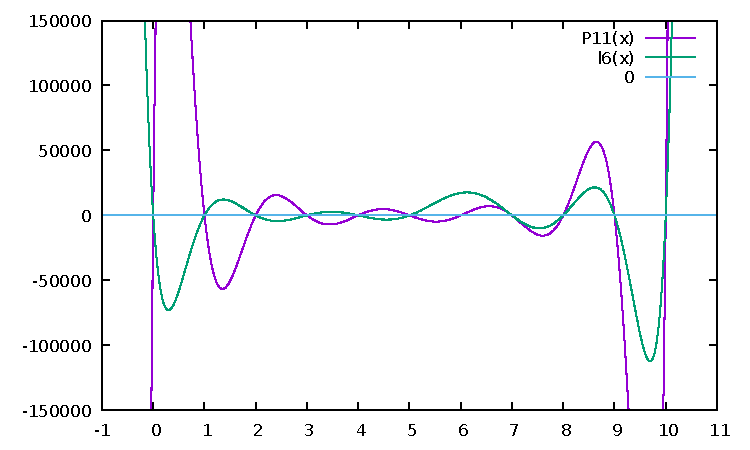
\includegraphics[height=0.5\textheight]{f/newtonlagrange.pdf}
\end{frame}

\begin{frame}
POINTS ÉQUIDISTANTS VS. POINTS DE TCHEBYCHEV\\
============================================

Points équidistants:
\[
	\frac1{n\sqrt{n}}\left(\frac{b-a}e\right)^{n+1}
	\le
	\left\|
	\Pi_{n+1}
	\right\|_\infty
	\le
	\frac{C}{\ln n\sqrt{n}}\left(\frac{b-a}e\right)^{n+1}
\]

Points de Tchebychev:
\[
	\left\|
	\Pi_{n+1}
	\right\|_\infty
	\le
	{C}\left(\frac{b-a}4\right)^{n+1}
\]

\end{frame}

\begin{frame}
CONSTANTE DE LEBESGUE\\
=====================

Norme~$\Lambda_n$ de l'opérateur
d'interpolation $P_n:\mathcal{C}([a,b])\to\R_n[X]$.
On a
\(
	\Lambda_n=\sup_{x\in[a,b]}\sum_{i=0}^n\left|\ell_i(x)\right|
\)

Points équidistants:
\[
	\Lambda_n\approx \frac{2^{n+1}}{e n\ln n}
\]

Points de Tchebychev:
\[
	\Lambda_n\approx \frac2\pi\ln n
\]

{\bf Corollaire.} Il existe une fonction continue~$f$ pour laquelle la suite
des~$P_n(f)$ diverge.
\end{frame}

\begin{frame}
RAPPEL: APPROXIMATION POLYNOMIALE (cours 2)\\
===========================================

{\bf Proposition 1.} (meilleure approximation uniforme)\\
Soit~$f\in\mathcal{C}([a,b])$.  Alors pour tout~$n\in\textbf{N}$ il existe un
unique~$Q_n(f)\in\R_n[X]$ tel que
\[
	\left\|Q_n(f)-f\right\|_\infty
	=
	\inf_{Q\in\R_n[X]}\left\|Q-f\right\|_\infty
\]

\pause

(Pas d'algorithme pour construire~$Q_n(f)$.)
\pause

Construction explicite d'une suite approximante pour~$f\in\mathcal{C}([0,1])$
(polynômes de Bernstein):
\[
	B_n(f)(p) =
	\sum_{k=0}^n
	f\left(\tfrac{k}{n}\right)
	{n\choose k}
	p^k(1-p)^{n-k}
\]
\end{frame}

\begin{frame}
RAPPEL: APPROXIMATION QUADRATIQUE (cours 2)\\
===========================================

{\bf Proposition 2.} (meilleure approximation quadratique)\\
Soit~$f\in L^2_\omega(]a,b[)$.  Alors pour tout~$n\in\textbf{N}$ il existe un
unique~$Q_n(f)\in\R_n[X]$ tel que
\[
	\left\|Q_n(f)-f\right\|_2
	=
	\inf_{Q\in\R_n[X]}\left\|Q-f\right\|_2
\]

{\bf Algorithme.} Projection orthogonale sur~$\R_n[X]$.

Calcul effectif avec polynômes orthogonaux en~$L^2_\omega(]a,b[)$.

\end{frame}

\begin{frame}
POLYNÔMES ORTHOGONAUX\\
=====================

Soit~$\omega:]a,b[\to\R$ un \emph{poids} positif et à moments finis.\\
On se place dans l'espace de Hilbert~$L^2_\omega(]a,b[)$.

{\bf\color{red} Exercice 15.}\\
1. Montrez qu'il existe une unique suite~$P_n$ de polynômes unitaires avec~$\mathrm{deg}(P_n)=n$ et~$P_n\perp\R_{n-1}[X]$.\\
2. Montrez que les racines de~$P_n$ sont simples et en~$]a,b[$.\\
{\bf\color{red}3.} Trouvez une récurrence~$P_n=(X-\lambda_n)P_{n-1}+\mu_nP_{n-2}$\\
{\bf\color{red}4.} Démontrez que les racines de~$P_n$ et~$P_{n+1}$ sont intercalées.

{\bf\color{red} Exercice H.} étude détaillée des polynômes d'Hermite
(voir pièce jointe)\\

\end{frame}



\begin{frame}
INTÉGRATION NUMÉRIQUE (COURS 3)\\
===============================

{\bf Problème~:} Étant donnée $f:[a,b]\to\R$ continue, calculer son
intégrale~$\int_a^b f(x)\d x$

{\bf Idée de base:} $\int_a^b f(x)\d x\ \approx\ \sum_{i=0}^n \lambda_i f(x_i)$

{\bf Méthode classique 1 (Newton-Cotes): }
Fixer les~$x_i\in[a,b]$; ensuite choisir les~$\lambda_i\in\R$ pour que
l'intégration soit exacte pour~$f\in\R_p[X]$ avec~$p$ le plus grand possible.

{\bf Méthode classique 2 (Gauss): }
Choisir les~$x_i\in[a,b]$ et les~$\lambda_i\in\R$ afin que
l'intégration soit exacte pour~$f\in\R_p[X]$ avec~$p$ le plus grand possible.

Le nombre~$p$ s'appelle l'{\bf ordre} de la méthode.

\end{frame}

\begin{frame}
INTÉGRATION NUMÉRIQUE (CONTEXTE)\\
===============================

En 2020, en pratique, le problème de l'intégration numérique en dimension 1 se
pose rarement.  On peut évaluer~$f(x)$ sur un million de points et faire la
somme instantanément.

La théorie de l'intégration numérique est néanmoins intéressante car il y a
beaucoup de résultats et techniques fondamentales associées (polynômes
orthogonaux, accélération de convergence).

L'intégration numérique en dimension élevée reste toujours un problème
difficile, que l'on traite souvent par des méthodes probabilistes (e.g.,
méthode de Monte-Carlo).

\end{frame}

\begin{frame}
ORDRE D'UNE MÉTHODE\\
===================

Considérons une méthode d'intégration~$I:\mathcal{C}([a,b])\to\R$.

{\bf Définition.}  On dit que~$I$ est d'ordre au moins~$N$ si
\[
	I(P)=\int_a^b P(x)\d x
	\qquad\forall P\in\R_N[X]
\]
et qu'elle est d'ordre~$N$ si elle est d'ordre au moins~$N$ mais pas d'ordre au moins~$N+1$.

L'erreur d'une méthode~$I$ pour une fonction~$f$ est
\[
	E(f)=\int_a^b f(x)\d x-I(f)
\]
\end{frame}

\begin{frame}
MÉTHODE DE NEWTON-COTES\\
=======================

Méthode de Newton-Cotes de rang~$n$:

On prend~$x_i=a+i\frac{b-a}{n}$ et~$\lambda_i=\int_a^b\ell_i(x)\d x$.  C'est à
dire~$I(f)=\sum_i \lambda_i f(x_i)$ est l'intégrale du polynôme interpolateur de~$f$ sur des points
équidistants.

{\bf\color{red} Exercice 16.}  Montrer que Newton-Cotes de rang~$n$ est d'ordre au moins~$n$ si~$n$ es impair, et d'ordre au moins~$n+1$ si~$n$ est pair.

{\bf\color{red} Exercice 17.} Soit~$E_n(f)$ l'erreur de Newton-Cotes de
rang~$n$, alors on a
\[
	|E_n(f)|\le\begin{cases}
		\frac{(b-a)^{n+2}}{(n+1)!}\left\|f^{(n+1)}\right\|_\infty
		& f\in\mathcal{C}^{n+1} \\
		\frac{(b-a)^{n+3}}{(n+1)!}\left\|f^{(n+2)}\right\|_\infty
		& f\in\mathcal{C}^{n+2},\ \textrm{$n$ pair} \\
	\end{cases}
\]
\end{frame}

\begin{frame}
FORMULES COMPOSITES\\
===================

{\bf Idée:} Subdiviser l'intervalle~$[a,b]$ en~$m$ parties égales, puis
calculer ~$I_n(f)$ sur chaque partie.

{\bf Formule:} On pose~$h=(b-a)/m$ et~$a_i=a+ih$, on définit
\[
	I_n^h(f)=\sum_{i=0}^{m-1} I_n^{[a_i, a_{i+1}]}(f)
\]
avec Newton-Cotes de rang~$n$ sur chaque partie~$[a_i, a_{i+1}]$.

{\bf\color{red} Exercice C. (prop.10)}\\
1. Démontrez
que~$|E_n^h(f)|\le(b-a)\frac{h^{n+1}}{(n+1)!}\left\|f^{(n+1)}\right\|_\infty$\\
2. Discutez la précision de~$I^h_n$ selon si~$n$ ou~$m\to\infty$.\\
3. Essayez une généralisation de~$I^h_n$ à dimension~$2$.\\
4. Essayez une généralisation de~$I^h_n$ à dimension~$d$, et évaluez la
précision selon si~$m$ ou~$n$ croit.
\end{frame}

\begin{frame}
MÉTHODE DE GAUSS\\
================

On veut approcher~$\int_a^b f(x)\omega(x)\d x$
par~$I_w(f)=\sum_i\lambda_if(x_i)$

{\bf Proposition 11.}
Étant donné~$n\in\N$, il existe un unique choix de points~$x_0,\ldots,x_n$ et
des coefficients~$\lambda_0,\ldots,\lambda_n$ pour que la méthode soit
d'ordre au moins~$N=2n+1$.  Les~$x_i$ sont les racines du polynôme ~$\omega$
orthogonal~$P_{n+1}$.

{\color{red}\bf Exercice 18.}\\
1. Démontrez que si la méthode est d'ordre au moins~$2n+1$, alors les~$x_i$ et les~$\lambda_i$ sont imposés.\\
2. Démontrez que ce choix donne bien une méthode d'ordre au moins~$2n+1$.

Indication: faire intervenir~$\Pi_{n+1}$.
\end{frame}

\begin{frame}
ERREUR DE PEANO\\
================

Soit~$E(f)=\int_a^b f(x)\omega(x)\d x-I_\omega(f)$.
Le {\bf noyau de Peano} d'ordre~$N$ est~$K_N(t)=E(x\mapsto(x-t)^N_+)$.

{\bf Proposition 12.} Si la méthode est d'ordre au moins~$N$
et~$f\in\mathcal{C}^{N+1}$ alors
\[
	E(f)=\frac{1}{N!}\int_a^b K_N(t)f^{(N+1)}(t)\d t
\]
Si de plus~$K_N$ est de signe constant alors il existe~$\xi\in]a,b[$ tel que
\[
E(f)=\frac{f^{(N+1)})(\xi)}{(N+1)!}E(x\mapsto x^{N+1})
\]

\vspace{-.5em}
{\bf\color{red} Exercice 19.}  Démontrez ces formules d'erreur de Peano.\\
{\bf\color{red} Exercice 20.}  Calculez le noyau de Peano pour~$n=0,2$.
\end{frame}

\begin{frame}
ACCÉLÉRATION DE CONVERGENCE\\
===========================

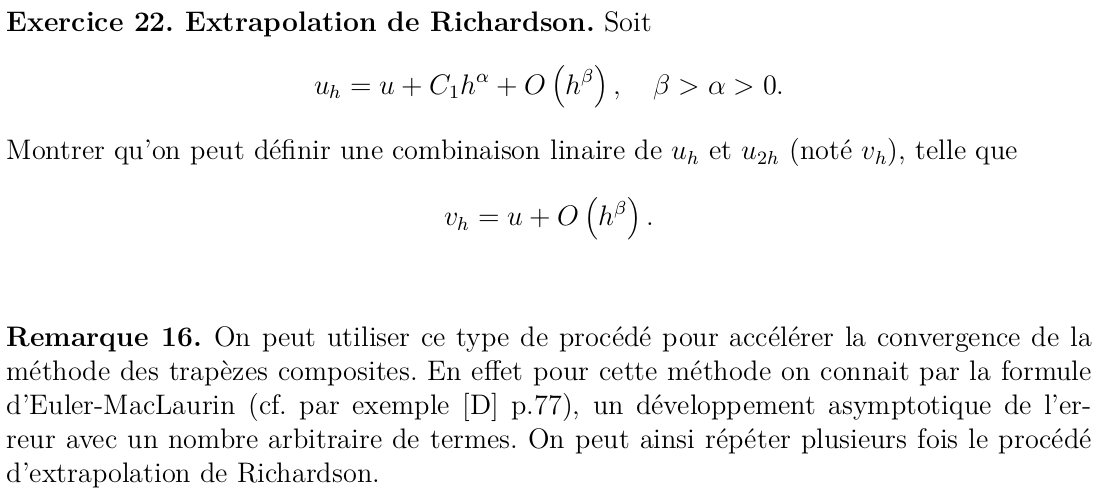
\includegraphics[width=\linewidth]{f/richardson.png}
\end{frame}

\begin{frame}
REPARTITION DES EXERCICES\\
=========================

{\bf Groupe 1.} Exercice 15\\
{\bf Groupe 2.} Exercice H\\
{\bf Groupe 3.} Exercices 16, 17\\
{\bf Groupe 4.} Exercice C\\
{\bf Groupe 5.} Exercice 18\\
{\bf Groupe 6.} Exercice 19 (et 20)\\
{\bf Groupe 7.} Exercice 22 (avec la remarque 16)\\

\end{frame}

\end{document}


% vim:sw=2 ts=2 spell spelllang=fr:
